% !TEX root = paper.tex
% !TEX encoding = UTF-8 Unicode
% -*- coding: UTF-8; -*-
% vim: set fenc=utf-8
% !TEX spellcheck = en-US
%=================================================================
\section{Methods}
\label{sec:methods}
%=================================================================
%=================================================================
In this study, the visual scene is made of an unknown target at a random position and a noisy background (see Figure~\ref{fig:intro}). An agent controls a focal visual sensor that can move over the visual scene through saccades. In the implementation of such networks, we will follow the simplifying assumption that there is a separation between the inferences of  position and category in two respective pathways, namely the ``What'' and the ``Where'' pathways. The ``What'' pathway will be given from the literature and to test the validity of our hypothesis, it is necessary to find at least one function implementing the ``where'' network and that would be able to find the position of an object knowing only the degraded retinal image. Here, we describe the methods that we will follow to find that function, from the generative models (first external and then internal) to the actual implementation of that ``where'' pathway knowing a fixed ``what'' pathway. %
%There are however many shortcuts allowing to render the calculation amenable. This includes (i) sparse encoding, (ii) approximate inference through model separation, and (iii) sampling-based metric training. 
%------------------------------%
%: see Figure~\ref{fig:methods}
\begin{figure}[t!]%%[p!]
\centering{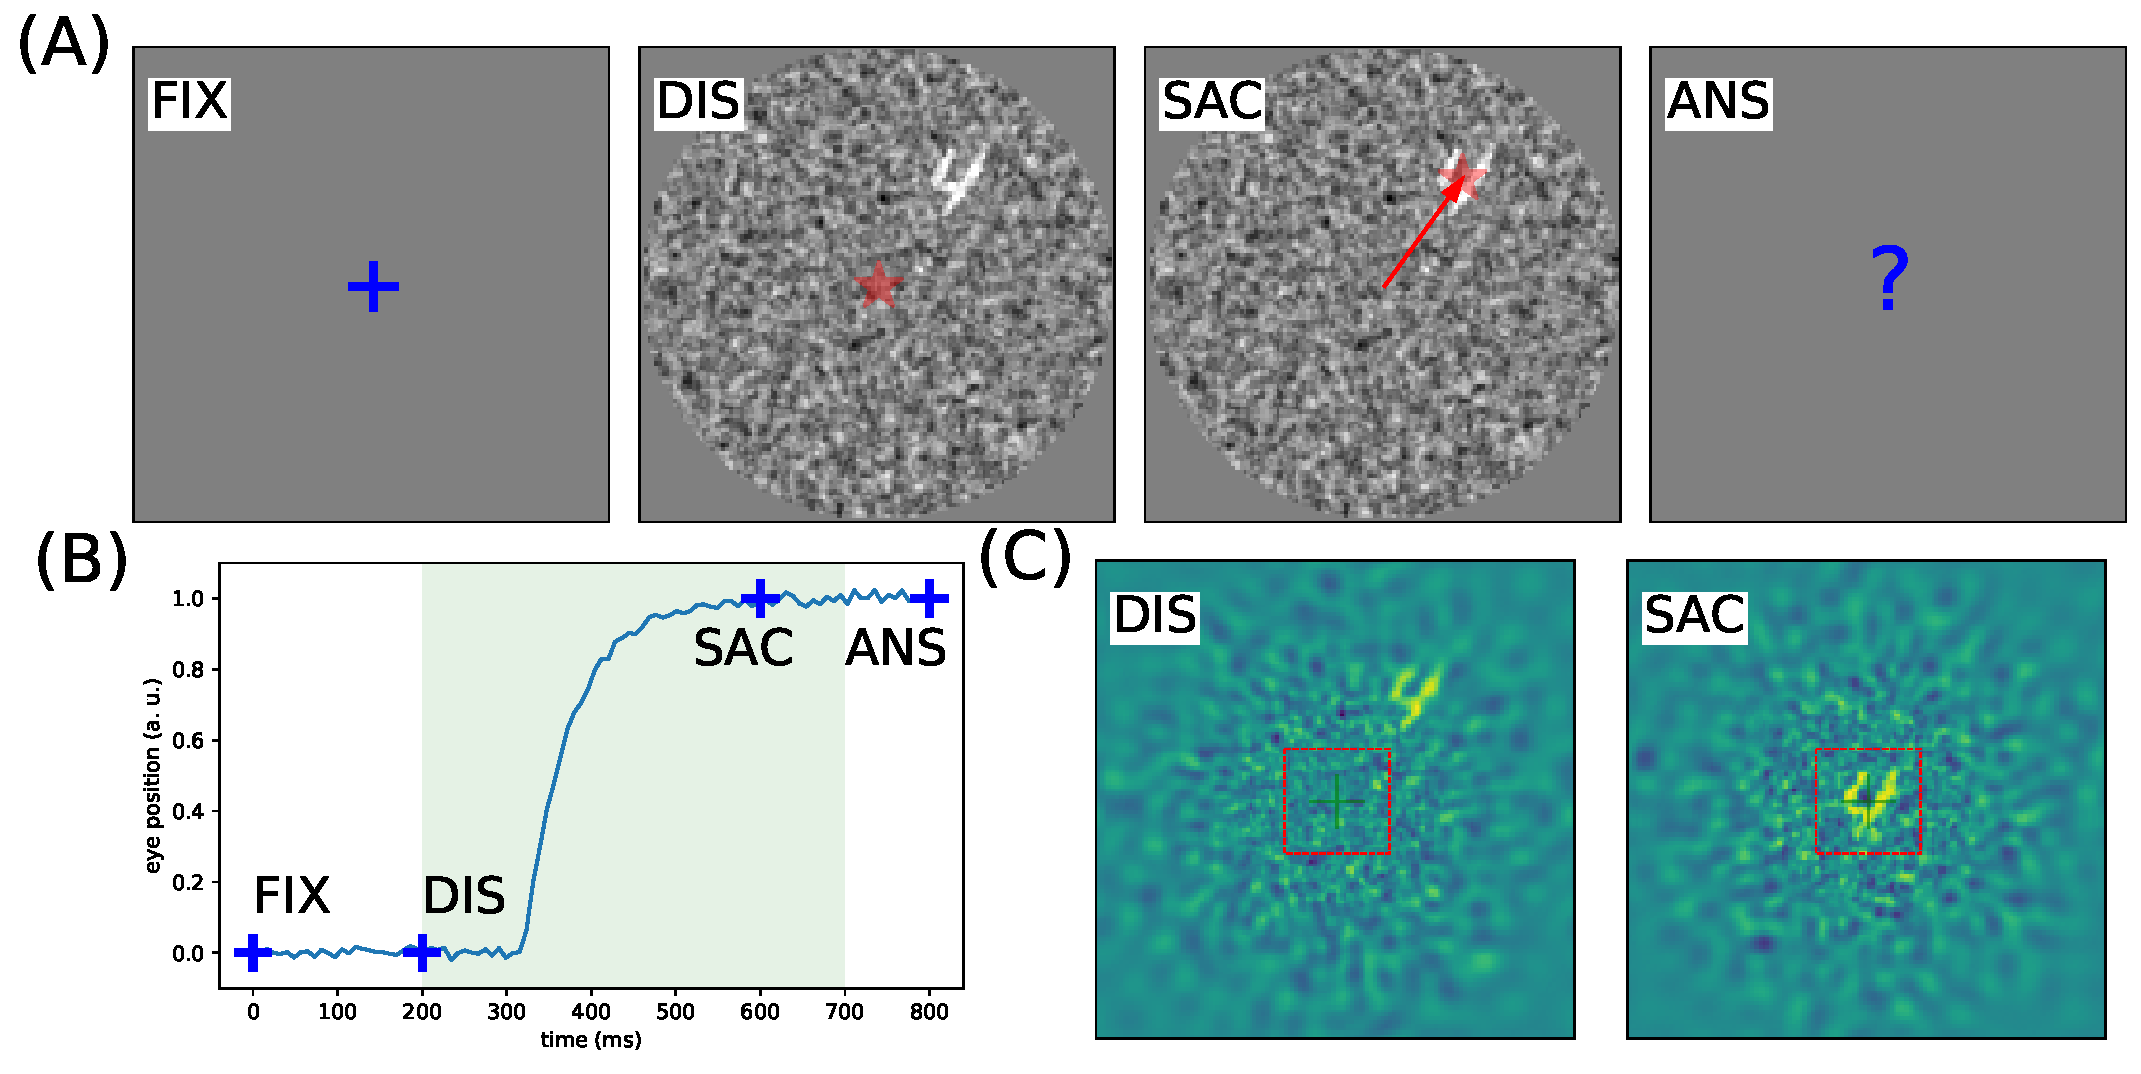
\includegraphics[width=\linewidth]{fig_intro}}%{fig_methods}}
\caption{
{\bf Methods for simulating active vision}:
\A We first define the model which generates images. It is composed of three different random processes: one choosing a sample image from the MNIST database (of size $28\times 28$) and placing it at a random position within the circular mask on the $128\times 128$ display. Then, this image is rectified and multiplied by a contrast factor and finally embedded in a natural-like noise with characterized by the noise contrast, mean spatial frequency and bandwidth~\citep{Sanz12}. %
\B The full-sized images are transformed into a retinal image which will be fed to the ``where'' pathway. This is implemented by a bank of filters whose centers are positioned on a log-polar grid and whose radius increases proportionally with eccentricity. In addition, a similar topographic map is used to represent the accuracy of each hypothetical position of a saccade, as represented by the collicular map. %
\C The ``where'' pathway is implemented by a three-layered neural network consisting of the retinal input, two hidden layers with $1000$ units each and a collicular output. Each unit is associated with a ReLU non-linearity. To learn to associate the output of the network with the ground truth, supervised training is performed using back-propagation with a binary cross entropy loss. This scalar measures the distance between both distributions (it is always positive and null if and only if they are equal). The network learns in about $20$ epochs as shown by the decrease of the loss function. Overlaid is the associated accuracy of the full active agent. This is computed by classifying the foveal image using the ``what'' pathway, after centering the gaze using the result of the ``where pathway''. This shows a gradual increase in accuracy from the baseline ($10\%$) to approximately an average of $X80.0X\%$. %
}%
\end{figure}%
%%------------------------------%
%
\subsection{Exteroceptive Generative model}
%=================================================================
It is first necessary to quantitatively define the generative model for input display images as shown first in Figure~\ref{fig:intro}-A (\DIS ) and as implemented in Figure~\ref{fig:methods}-A. 

\paragraph{Targets.} Following a common hypothesis regarding active vision, visual scenes will consist of a single visual object of interest. We will use the MNIST database of handwritten digits introduced by~\citep{Lecun1998}. Indeed, we are here focused on the problem of localization (``where'' pathway) and classification solutions (``what'' pathway) abound for this class of targets. Samples are drawn from a database of $60000$ grayscale $28\times 28$ pixels images and separated between a training and a validation set (see below the description of the ``where'' network). 
\paragraph{Full-scale images.} For each sample, we may now draw a random position in a full-scale image of $128\times 128$. To enforce isotropic saccades, we define a centered circular mask covering the image (of radius $64$ pixels) and the position is such that the embedded sample fits entirely into that circular mask.
\paragraph{Background noise setting. } To provide with a realistic background noise, we generated synthetic textures~\citep{Sanz12} using a third random process. These textured images are of the same size of the full-image. These static images are designed to fit well with the statistics of natural images. We chose an isotropic setting where textures are characterized by solely two parameters. One controls the median spatial frequency $sf_0$ of this noise, while the other controls the bandwidth around this central spatial frequency. Equivalently, these can be considered as the band-pass filtering of random white noise images. Finally, these images are rectified to have a normalized contrast.
\paragraph{Adding signal and noise. } Finally, both the noise and the target image are merged into a single image. We have used two different strategies. In a first strategy emulating a transparent association, we computed the average luminance at each pixel, while in a second strategy emulating an opaque association, we choose for each pixel the maximal value. The quantitative difference were tested in simulations, but proved to have a marginal importance.
%
\subsection{Interoceptive generative model}
%=================================================================
%
We will now define the simplified anatomy of our agent, which is composed of two separate pathways.
\paragraph{Foveal vision and the ``what'' pathway}
First, foveal vision is defined as the $28\times 28$ pixels image centered at the point of fixation (see dashed red box in Figure~\ref{fig:intro}-C). This image is then directly passed to the agent's visual categorical pathway (the ``What'' pathway). This is realized by the known ``LeNet'' classifier~\citep{Lecun1998}, that processes the $28 \times 28$ central pixels to identify the target category. Such a network is directly provided (and unmodified) by the pyTorch library~\citep{Paszke17}, and consists of a 3-layered Convolutional Neural Network. It is trained over the (centered) MNIST database after approx $20$ training epochs. Input images are rectified (with a mean and standard deviation of respectively $0.1307$ and $0.3081$). The network outputs a vector representing the probability of detecting each of the $10$ digits. We use the argument of the output neuron with maximum probability, to categorize each image. This strategy achieves an average $98.7\%$ accuracy on the validation dataset~\citep{Lecun1998}. % 

\paragraph{Retinal transform: Peripheral vision and log Polar encoding}
First, both the visual features and the expected target position may to be expressed in retinal coordinates which we choose here to be log-polar as it provides a good fit with observations in mammals~\citep{Traver10}. On the visual side, we extracted local visual features as oriented edges  as the combination of the retinotopic transform with that of the primary visual cortex~\citep{Fischer2007a}. The centers of these first and second order orientation filters are radially organized around the center of fixation, with small and tightened receptive fields at the center and more large and scarce receptive fields at the periphery, see  Figure~\ref{fig:methods}-B. The size of the filters increases proportionally to eccentricity. The filters are organized in $10$ spatial eccentricity scales (respectively placed at around $2$, $3$, $4.5$, $6.5$, $9$, $13$, $18$, $26$, $36.5$ , and $51.3$ pixels from the center) allowing them to cover most of the original $128 \times 128$ image.  At each of these position, we computed $16$ different orientations and $2$ different phases (symmetric and anti-symmetric) using log-Gabor filters~\citep{Fischer2007a}. This finally implements a (fixed) bank of linear filters which model the receptive fields of the input to the primary visual cortex.

From any input image ($128\times 128=16384$ pixels) is linearly transformed into a retinal activity vector $\boldsymbol{x}$. In practice, the length of this vector is $1600$ such that the retinal filter compresses the original image by about 90\%, with high spatial frequencies preserved at the center and only low spatial frequencies conserved at the periphery. In practice, this filters are pre-computed and placed into a matrix for a rapid transform of batches of input displays into retinal transforms. In practice this matrix transformation allows also the evaluation of a reconstructed visual image given a retinal activity vector thanks to the pseudo-inverse matrix of the forward transform matrix. In summary, the full-sized images are transformed into a peripheral retinal image which will be fed to the ``where'' pathway.

\paragraph{Collicular representation: Metric training}
% >>> Laurent is here <<<

 In particular, we could also evaluate after this training phase the accuracy map of the classifier knowing a translational shift imposed to the input image. 

 Crucially, a similar transform is used to compute the accuracy of each hypothetical saccade, as represented by the collicular map. %


%The target accuracy map is also organized radially in a log-polar fashion, making the target position estimate more precise at the center and fuzzier at the periphery. This modeling choice is reminiscent of the approximate log-polar organization of the superior colliculus (SC) motor map {\bf[TODO:REF]}.
%This retinotopic organization is preserved along the visuo-motor pathway as expected from observations {\bf[TODO:REF]}.

 This central classifier displays a high accuracy at the center, and a fast decreasing accuracy with target eccentricity, as shown in figure \ref{fig:results}-D. In contrast, the visual orientation pathway (the ``Where'' pathway) takes the full visual field into account in order to tell whether a target is present at the different peripheral locations, in order to monitor future saccades.




\subsection{Implementing the ``where'' pathway}
%=================================================================

\paragraph{Active inference}
%Second, we %start as in~\citep{Friston12} by a probabilistic formulation, and 
To implement the ``where pathway'', we will use the fundamental hypothesis outlined in Figure~\ref{fig:intro}: the position of an object is independent from its category.  This allows considering $u$ and $y$ being independently inferred from the current visual field, i.e $p(U,Y|x) = p(U|x) p(Y|x)$. This property is strictly true in our setting and is very generic in vision for simple classes (such as digits) and simple displays (but see~\citep{Vo12} for more complex visual scene grammars). 
From this independence hypothesis, we may separate both inferences (identification vs localization) in two separate pathways with different morphologies (respectively foveal and peripheral). Note that from the retinotopic projection of the visual information, this independence is conditional on action: both pathways should update their beliefs upon decisions made in each respective pathway {\bf (??)}.
%A first simplifying assumption is a separation of the position and category inferences in two separate pathways, namely the ``What'' and the ``Where'' pathways.
The agent visual categorical pathway (the ``What'' pathway) is supposed to be realized by the known ``LeNet'' classifier~\citep{Lecun1998}, that processes the $28 \times 28$ central pixels to identify the target category (see dashed red boxes in  Figure~\ref{fig:intro}-C). This central classifier displays a high accuracy at the center, and a fast decreasing accuracy with target eccentricity, as shown in figure \ref{fig:results}-D. In contrast, the visual orientation pathway (the ``Where'' pathway) takes the full visual field into account in order to tell whether a target is present at the different peripheral locations, in order to monitor future saccades.


This fundamental hypothesis was outlined in Figure~\ref{fig:intro}: the position $u$ of an object is independent from its category (identity) $y$. This allows considering $u$ and $y$ being independently inferred from the current visual field, i.e $p(U,Y|x) = p(U|x) p(Y|x)$. This property is strictly true in our setting and is very generic in vision for simple classes (such as digits) and simple displays (but see~\citep{Vo12} for more complex visual scene grammars). 
From this independence hypothesis, we may separate both inferences (identification vs localization) in two separate pathways with different morphologies (respectively foveal and peripheral). Note that from the retinotopic projection of the visual information, this independence is conditional on action: both pathways should update their beliefs upon decisions made in each respective pathway.
To check this hypothesis, we train a multi-layer neural network to predict accuracy maps from a retinotopic log-polar encoding of the visual image. 

Active inference assumes a hidden emitter $e$, which is known indirectly through its effects on the sensor, that obey to a generative process : $x\sim p(X|e)$. The real emitter state $e$ being hidden, a parametric model $\theta$ is assumed to allow estimate the cause of the current visual field through model inversion thanks to Bayes formula, in short:
$$p(E|x) \propto p(x|E;\theta)$$
with $x$ the visual field in our case. Assume now that the cause $e$ of the visual field splits in two (independent) components, namely $e = (u,y)$ with $u$ the body posture (in our case the gaze orientation) and $y$ the object shape (or object identity). Assume also that a set of motor commands $A = \{..., a, ...\}$ may control the body posture, but not the object's identity, so that $y$ is invariant to $a$.
Then, before taking a decision, the consequence of every saccade should be analyzed  through model inversion \emph{over the future observations}, that is predicting the effect of every $a$ in $A$ to choose the action that may optimizes future inferences. The benefit of each $a$ is quantified through a certain metric (future accuracy, future posterior entropy, future variational free energy, ...), that depend on the current inference $p(U,Y|x)$. Each saccade $a$ is thus expected to provide a new visual sample from a given scene statistics, which may increase the understanding of the scene (here the target position and category). However, estimating the effect of every action over the range of every possible object shapes and body postures is combinatorially hard, even in simple cases such as vision, and thus infeasible in practice. 


Though the effect of action is too complex to be inferred from a generative model, we assume here that it is trained by sampling, i.e. by "trial and error". There are however many shortcuts allowing to render the calculation amenable. This includes (i) sparse encoding, (ii) approximate inference through model separation, and (iii) sampling-based metric training. 


\paragraph{Metric training}
%=======
%>>>>>>> 10eba6746a264a8f6141953d7948057e5093489d
Third, the putative effect of every saccade should be condensed in a single number, the \emph{accuracy}, that is the expected benefit of issuing saccade $a$ %regarding the target identity, both assuming $p(U|\boldsymbol{x})$ and $p(Y|\boldsymbol{x})$ 
from the current observation. Taking $a$ a possible saccade and $\tilde{\boldsymbol{x}}$ the corresponding future visual field, the result of the categorical classifier over $\tilde{\boldsymbol{x}}$ can either be correct (1) or incorrect (0). 
If this experiment is repeated many times over many visual scenes, the probability of correctly classifying the future visual field $\tilde{\boldsymbol{x}}$ after a saccade $a$ forms a probability, i.e. a number between 0 and 1, that reflects the proportion of correct and incorrect classifications.
% when issuing a saccade $a$ after seeing $\boldsymbol{x}$ (the initial visual field). 
It more or less corresponds to inferring the true target identity $\hat{y}$, i.e. $p(\hat{y}|\tilde{\boldsymbol{x}})$, including the update of the eye direction, that is a sample of the ``real'' generative process. Active inference needs either the current identity $y$ or the current eye direction $u$ to be readable from the present view, in order to effectively predict future inferences, through computationally intensive predictions.   
Instead of doing predictions from a generative model, better off is to form a statistics over the (scene understanding) benefit obtained from past saccades in the same context, that is forming an \emph{accuracy map} from the current view. This is the essence of \emph{sampling-based metric prediction}.

In detail, the primary visual field should be transformed so as to predict how accurate the categorical classifier will be after the saccade is carried out~\citep{Dauce18}. %The set of all possible saccade predictions should 
An accuracy map abstracts here a full sequence of operations, including ($i$) an initial visual examination, followed by ($ii$) a decision, ($iii$) a saccade realization and ($iv$) a second visual examination that should finally ($v$) determine the category of the target.
It should be mostly organized radially, preserving the initial retinotopic organization, with high predicted accuracies reflecting a high probability of target presence at given locations.
Such a \emph{predictive accuracy map} is assumed to be the core of a realistic saccade-based vision system, with action selection (motor map) overlaying the accuracy map through a winner-takes-all mechanism (as thought to be done in the superior colliculus). Of course, each different initial visual field comes with a different accuracy map (essentially conveying information about the target retinotopic position).
Our main argument is that such an accuracy map is trainable in a rather straightforward way, through trials and errors, by actuating saccades after processing the visual input, and taking the final classification success or failure as a teaching signal.




\paragraph{Approximate inference}
Active inference assumes a hidden emitter $e$, which is known indirectly through its effects on the sensor, that obey to a generative process : $x\sim p(X|e)$. The real emitter state $e$ being hidden, a parametric model $\theta$ is assumed to allow estimate the cause of the current visual field through model inversion thanks to Bayes formula, in short:
$$p(E|x) \propto p(x|E;\theta)$$
with $x$ the visual field in our case. Assume now that the cause $e$ of the visual field splits in two (independent) components, namely $e = (u,y)$ with $u$ the body posture (in our case the gaze orientation) and $y$ the object shape (or object identity). Assume also that a set of motor commands $A = \{..., a, ...\}$ may control the body posture, but not the object's identity, so that $y$ is invariant to $a$.
Then, before taking a decision, the consequence of every saccade should be analyzed through model inversion \emph{over the future observations}, that is predicting the effect of every $a$ in $A$ to choose the action that may optimizes future inferences. The benefit of each $a$ is quantified through a certain metric (future accuracy, future posterior entropy, future variational free energy, ...), that depend on the current inference $p(U,Y|x)$. Each saccade $a$ is thus expected to provide a new visual sample from a given scene statistics, which may increase the understanding of the scene (here the target position and category). However, estimating the effect of every action over the range of every possible object shapes and body postures is combinatorially hard, even in simple cases such as vision, and thus infeasible in practice. 





\paragraph{Classifier training}
Modern parametric classifiers are composed of many layers (hence the term ``Deep Learning'') that can be trained through gradient descent over arbitrary input and output feature spaces. The ease of use of those tightly optimized training algorithms allow to quantify the difficulty of a task through training failure or success. Consider the visual features $\boldsymbol{x}$ as the input and a log-polar retinotopic vector $\boldsymbol{a}$ made of $n$ Bernouilli probabilities (success probabilities) as the output. A textured background noise is used at the input so that (i) the target statistics should barely differ from that of the background and (ii) a categorical classifier may not be trainable with the initial view as the input. A training set is made of randomly generated noisy images, with a low-contrast $28\times 28$ MNIST character  {\bf [REF?]} randomly positioned around the center of fixation (at maximum $30$ pixels from the center of fixation). The images are first whitened {\bf [REF?]}, and then transformed through $16384$ oriented log-polar filters radially organized around the center of fixation, with tight receptive fields at the center and large receptive fields at the periphery. 

Each visual input is accompanied with a corresponding accuracy map also organized radially through $10$ eccentricity scales and $16$ peripheral directions. The training is done in Pytorch {\bf [REF?]}. The parametric neural network is made of two fully connected hidden layers of size $1000$, with ReLu activation and $50 \%$ drop-out on the last layer. The network is trained over $600,000$ saccades on full-images, using the binary cross-entropy loss as the error signal, with a learning rate equal to $10^{-4}$. The training is done in about $1$ hours on a laptop.


